\usepackage{graphicx}

\documentclass[a4paper, 14pt]{extarticle}

%%% Спасибо https://github.com/Amet13/bachelor-diploma/blob/master/inc/preamble.tex
%%% Преамбула %%%

\usepackage{fontspec} % XeTeX
\usepackage{xunicode} % Unicode для XeTeX
\usepackage{xltxtra}  % Верхние и нижние индексы
\usepackage{pdfpages} % Вставка PDF

\usepackage{listings} % Оформление исходного кода
\lstset{
basicstyle=\small\ttfamily, % Размер и тип шрифта
breaklines=true, % Перенос строк
tabsize=2, % Размер табуляции
literate={--}{{-{}-}}2 % Корректно отображать двойной дефис
}

% Шрифты, xelatex
\defaultfontfeatures{Ligatures=TeX}
\setmainfont{Times New Roman} % Нормоконтроллеры хотят именно его
\newfontfamily\cyrillicfont{Times New Roman}
%\setsansfont{Liberation Sans} % Тут я его не использую, но если пригодится
\setmonofont{FreeMono} % Моноширинный шрифт для оформления кода

% Русский язык
\usepackage{polyglossia}
\setdefaultlanguage{russian}

\usepackage{amssymb,amsfonts,amsmath} % Математика
\numberwithin{equation}{section} % Формула вида секция.номер

\usepackage{enumerate} % Тонкая настройка списков
\usepackage{indentfirst} % Красная строка после заголовка
\usepackage{float} % Расширенное управление плавающими объектами
\usepackage{multirow} % Сложные таблицы

% Пути к каталогам с изображениями
\usepackage{graphicx} % Вставка картинок и дополнений

% Формат подрисуночных записей
\usepackage{chngcntr}
\counterwithin{figure}{section}

% Гиперссылки
\usepackage{hyperref}
\hypersetup{
colorlinks, urlcolor={black}, % Все ссылки черного цвета, кликабельные
linkcolor={black}, citecolor={black}, filecolor={black},
}

% Оформление библиографии и подрисуночных записей через точку
\makeatletter
\renewcommand*{\@biblabel}[1]{\hfill#1.}
\renewcommand*\l@section{\@dottedtocline{1}{1em}{1em}}
\renewcommand{\thefigure}{\thesection.\arabic{figure}} % Формат рисунка секция.номер
\renewcommand{\thetable}{\thesection.\arabic{table}} % Формат таблицы секция.номер
\def\redeflsection{\def\l@section{\@dottedtocline{1}{0em}{10em}}}
\makeatother

\renewcommand{\baselinestretch}{1.4} % Полуторный межстрочный интервал
\parindent 1.27cm % Абзацный отступ

\sloppy             % Избавляемся от переполнений
\hyphenpenalty=1000 % Частота переносов
\clubpenalty=10000  % Запрещаем разрыв страницы после первой строки абзаца
\widowpenalty=10000 % Запрещаем разрыв страницы после последней строки абзаца

% Отступы у страниц
\usepackage{geometry}
\geometry{left=2cm}
\geometry{right=1cm}
\geometry{top=2cm}
\geometry{bottom=2cm}

% Списки
\usepackage{enumitem}
\setlist[enumerate,itemize]{leftmargin=1.82cm} % Отступы в списках

\makeatletter
\AddEnumerateCounter{\asbuk}{\@asbuk}{м)}
\makeatother
\setlist{nolistsep} % Нет отступов между пунктами списка
\renewcommand{\labelitemi}{--} % Маркет списка --
\renewcommand{\labelenumi}{\asbuk{enumi})} % Список второго уровня
\renewcommand{\labelenumii}{\arabic{enumii})} % Список третьего уровня

% Содержание
\usepackage{tocloft}
\renewcommand\cftsecafterpnum{\vskip0pt}
\renewcommand\cftsubsecafterpnum{\vskip0pt}
\setlength\cftbeforesecskip{0pt}
\setlength\cftbeforesubsecskip{0pt}

\renewcommand{\cfttoctitlefont}{\hspace{0.38\textwidth}\MakeTextUppercase} % СОДЕРЖАНИЕ
\renewcommand{\cftsecfont}{\hspace{0pt}}            % Имена секций в содержании не жирным шрифтом
\renewcommand\cftsecleader{\cftdotfill{\cftdotsep}} % Точки для секций в содержании
\renewcommand\cftsecpagefont{\mdseries}             % Номера страниц не жирные
\setcounter{tocdepth}{3}                            % Глубина оглавления, до subsubsection


%% Нумерация страниц справа сверху
%\usepackage{fancyhdr}
%\pagestyle{fancy}
%\fancyhf{}
%\fancyhead[R]{\textrm{\thepage}}
%\fancyheadoffset{0mm}
%\fancyfootoffset{0mm}
%\setlength{\headheight}{17pt}
%\renewcommand{\headrulewidth}{0pt}
%\renewcommand{\footrulewidth}{0pt}
%\fancypagestyle{plain}{
%\fancyhf{}
%\rhead{\thepage}
%}

% Формат подрисуночных надписей
\RequirePackage{caption}
\DeclareCaptionLabelSeparator{defffis}{ -- } % Разделитель
\captionsetup[figure]{justification=centering, labelsep=defffis, format=plain} % Подпись рисунка по центру
\captionsetup[table]{justification=raggedright, labelsep=defffis, format=plain, singlelinecheck=false} % Подпись таблицы слева

% Заголовки секций в оглавлении в верхнем регистре
\usepackage{textcase}
\makeatletter
\let\oldcontentsline\contentsline
\def\contentsline#1#2{
\expandafter\ifx\csname l@#1\endcsname\l@section
\expandafter\@firstoftwo
\else
\expandafter\@secondoftwo
\fi
{\oldcontentsline{#1}{\MakeTextUppercase{#2}}}
{\oldcontentsline{#1}{#2}}
}
\makeatother

% Оформление заголовков
\usepackage[compact,explicit]{titlesec}
\titleformat{\section}{}{}{12.5mm}{\clearpage\centering{\MakeTextUppercase{#1}}\vspace{24pt}}
\titleformat{\subsection}[block]{\vspace{0pt}}{}{12.5mm}{\thesubsection\quad\textbf{#1}\vspace{24pt}}
\titleformat{\subsubsection}[block]{\vspace{1em}\normalsize}{}{12.5mm}{\thesubsubsection\quad#1\vspace{1em}}
\titleformat{\paragraph}[block]{\normalsize}{}{12.5mm}{\MakeTextUppercase{#1}}

\titlespacing*{\section}
{0pt}{5.5ex plus 1ex minus .2ex}{4.3ex plus .2ex}
\titlespacing*{\subsection}
{0pt}{5.5ex plus 1ex minus .2ex}{4.3ex plus .2ex}

% Секции без номеров (введение, заключение...), вместо section*{}
\newcommand{\anonsection}[1]{
\clearpage
\phantomsection % Корректный переход по ссылкам в содержании
\paragraph{\centerline{{#1}}\vspace{1.5em}}
\addcontentsline{toc}{section}{\uppercase{#1}}
}

% Секции для приложений
\newcommand{\appsection}[1]{
\phantomsection
\paragraph{\centerline{{#1}}}
\addcontentsline{toc}{section}{\uppercase{#1}}
}

% Библиография: отступы и межстрочный интервал
\makeatletter
\renewenvironment{thebibliography}[1]
{\section*{\refname}
\list{\@biblabel{\@arabic\c@enumiv}}
{\settowidth\labelwidth{\@biblabel{#1}}
\leftmargin\labelsep
\itemindent 16.7mm
\@openbib@code
\usecounter{enumiv}
\let\p@enumiv\@empty
\renewcommand\theenumiv{\@arabic\c@enumiv}
}
\setlength{\itemsep}{0pt}
}
\makeatother

\usepackage[figurename=Рисунок]{newfloat} %Floating environments
\DeclareGraphicsExtensions{.pdf,.png,.jpg}
\graphicspath{{images/pdf/}{images/png/}{images/jpg/}}


\usepackage[outputdir=\detokenize{../out/}, newfloat=true]{minted}
\setminted[cpp]{
linenos=true,
breaklines=true,
encoding=utf8,
frame=single,
fontsize=\small,
tabsize = 2
}


\usepackage[parentracker=true,
backend=biber,
hyperref=auto,
language=auto,
autolang=other,
citestyle=gost-numeric,
defernumbers=true,
bibstyle=gost-numeric,
]{biblatex}

% Russian sources first
\DeclareSourcemap{
\maps[datatype=bibtex]{
\map{
\step[fieldset=langid, fieldvalue={tempruorder}]
}
\map[overwrite]{
\step[fieldsource=langid, match=russian, final]
\step[fieldsource=presort, match=\regexp{(.+)}, replace=\regexp{aa$1}]  %$
}
\map{
\step[fieldsource=langid, match=russian, final]
\step[fieldset=presort, fieldvalue={az}]
}
\map[overwrite]{
\step[fieldsource=langid, notmatch=russian, final]
\step[fieldsource=presort, match=\regexp{(.+)}, replace=\regexp{za$1}]  %$
}
\map{
\step[fieldsource=langid, notmatch=russian, final]
}
\map{
\step[fieldsource=langid, match={tempruorder}, final]
\step[fieldset=langid, null]
}
}
}
%\xpatchbibmacro{related:default}
%  {\renewbibmacro*{pageref}{}}
%  {\renewbibmacro*{pageref}{}\renewbibmacro*{begentry}{}}{}{}
%\renewbibmacro*{begentry}
%  {\hspace{-4em}\makebox[4em]{\hyperlink{\thefield{entrykey}}{$\Downarrow$}}%
%       \raisebox{\baselineskip}{\hypertarget{back:\thefield{entrykey}}{}}}%
\edef\mytempforAtCharacter{\char64}
\def\getkey#1#2{%
\csappto{mytempforbibkey}{#1}%
\ifstrequal{#2}{,}
{\hspace{-4em}\makebox[4em]{\hyperlink{back:\mytempforbibkey}{$\Uparrow$}}%
\raisebox{\baselineskip}{\hypertarget{\mytempforbibkey}{}}%
\mytempforAtCharacter\mytempforbibtype\{\mytempforbibkey,}
{\getkey#2}%
}
\renewcommand*{\do}[1]{\csdef{#1}##1{\def\mytempforbibtype{#1}\def\mytempforbibkey{}\getkey}}
\docsvlist{MVBOOK,BOOK,INBOOK,SUPPBOOK,BOOKINBOOK,MVCOLLECTION,COLLECTION,INCOLLECTION,SUPPCOLLECTION,MVREFERENCE,REFERENCE,INREFERENCE,MVPROCEEDINGS,PROCEEDINGS,INPROCEEDINGS,PERIODICAL,ARTICLE,PATENT,ONLINE,THESIS,mvbook,book,inbook,suppbook,bookinbook,mvcollection,collection,incollection,suppcollection,mvreference,reference,inreference,mvproceedings,proceedings,inproceedings,periodical,article,patent,online,thesis,Article,Book,MVBook,InBook,BookInBook,SuppBook,Booklet,Collection,MVCollection,InCollection,SuppCollection,Manual,Misc,Online,Patent,Periodical,SuppPeriodical,Proceedings,MVProceedings,InProceedings,Reference,MVReference,InReference,Report,Thesis,Unpublished}
\renewcommand*{\do}[1]{\csdef{#1}##1{\mytempforAtCharacter #1\{}}
\docsvlist{XDATA,COMMENT,xdata,comment,}

\setcounter{biburllcpenalty}{7000}
\setcounter{biburlucpenalty}{8000}
\addbibresource{sources.bib}

\begin{document}

	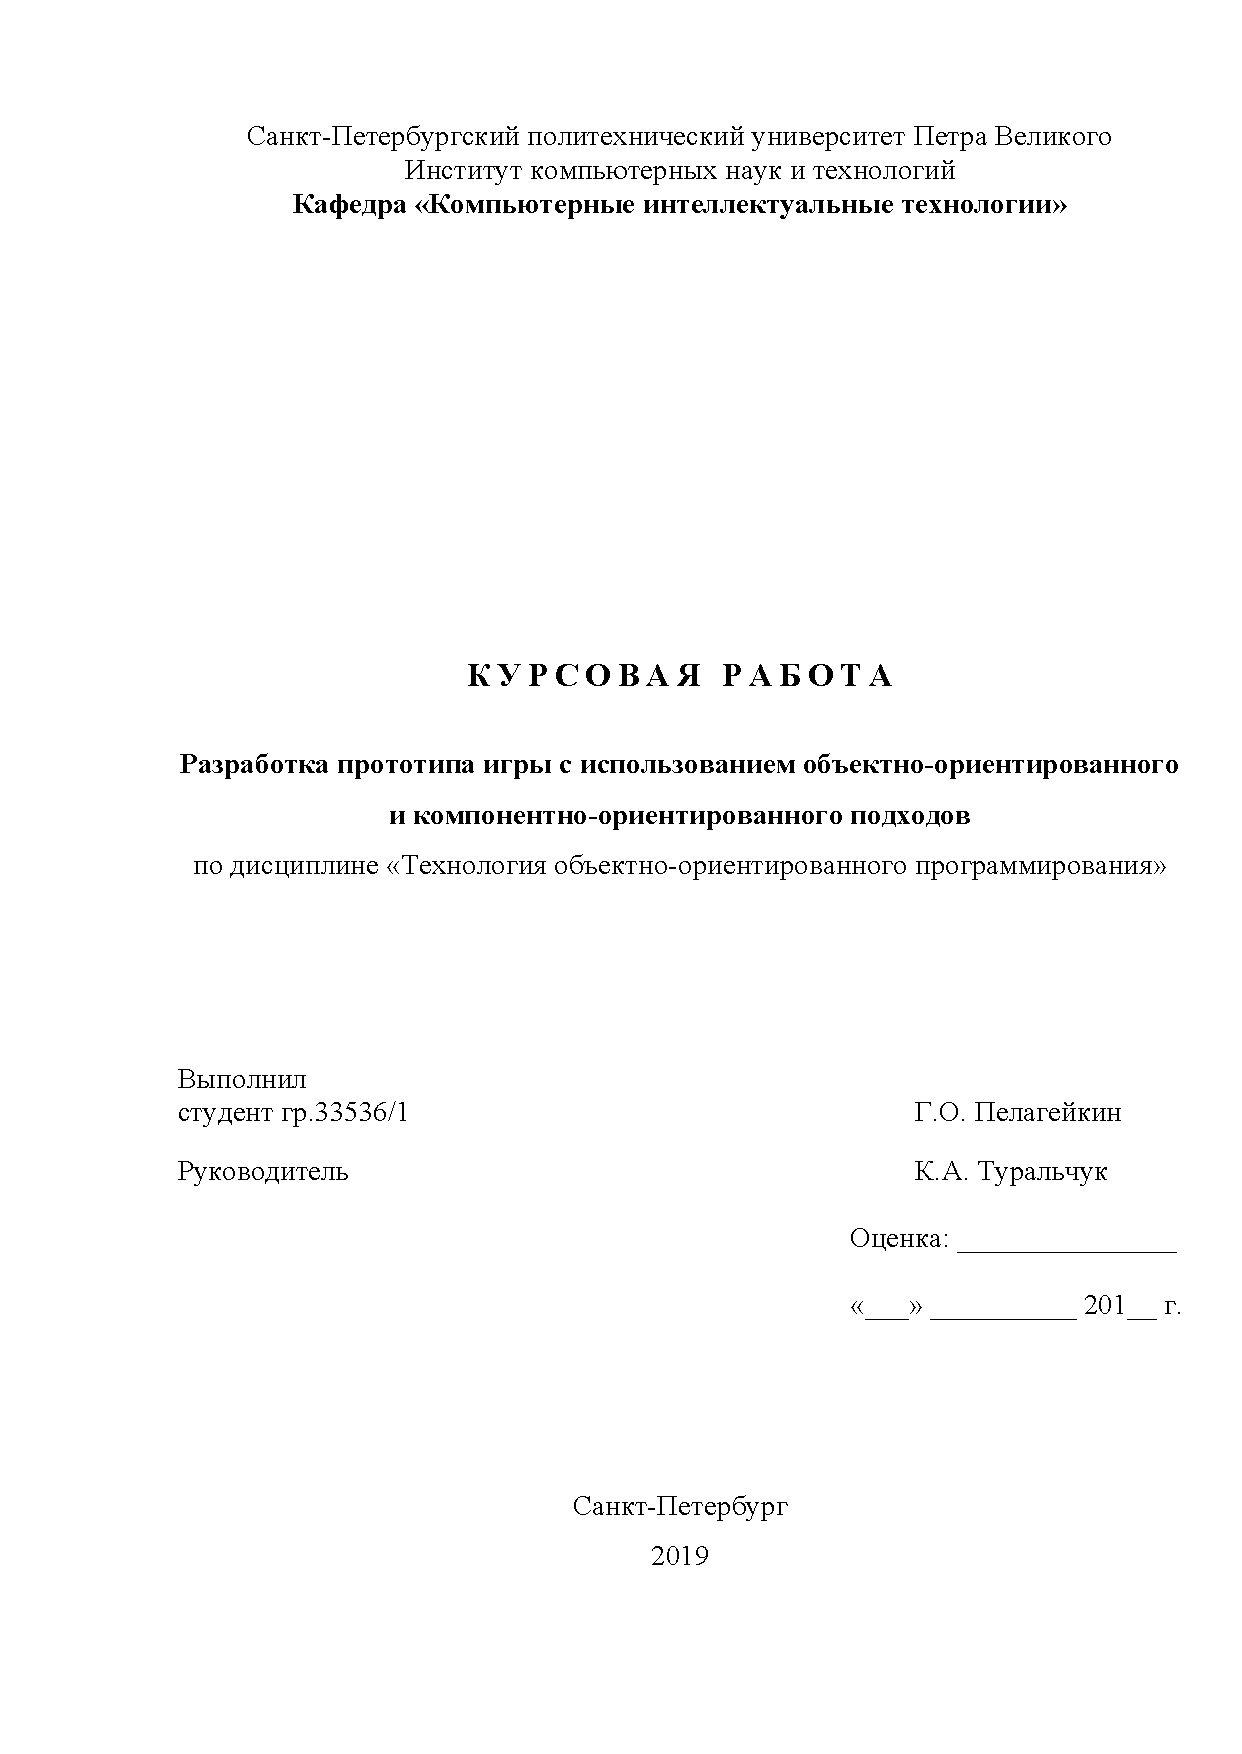
\includepdf{title-page}

	\tableofcontents

	\begin{anonsection}{Введение}
		В данной работе будет рассмотрен процесс создания простой игры.
		В качестве эталона взята логика игры <<Atomic Bomber>>, реализация будет выполнена на языке C++ на основе легковесного игрового движка Urho3D.
		В ходе выполнения работы будут выполнены следующие задачи:
		\begin{enumerate}
			\item Декомпозиция задачи.
			\item Реализация основных компонентов игры с использованием комбинации подходов объектно-ориентированного, компонентно-ориентированного и событийно-ориентированного программирования.
			\item Тестирование и отладка приложения.
		\end{enumerate}

		В результате должны быть закреплены и расширены навыки программирования с использованием выбранного набора программных средств и получен работающий прототип игры.

	\end{anonsection}

	\begin{section}{Обзор предметной области}

		\begin{subsection}{Постановка задачи}

			В качестве темы данной работы была выбрана реализация игры, повторяющей основные аспекты геймплея игры <<Atomic Bomber>> за авторством Luke Allen.
			Это двухмерная игра для мобильных устройств, работающая по простыми правилам, которые, тем не менее, формируют интересный игровой процесс.

			<<Atomic Bomber>> была выбрана в качестве эталона реализации игровой логики в данной работе, так как игровая логика максимально проста и может быть реализована за разумное время, но для ее корректной реализации потребуется применить различные техники программирования, которые будут рассмотрены далее.

			Приведем основные аспекты игровой логики, которые будут реализованы.

			\begin{enumerate}
				\item Игровой мир двухмерный, вид сбоку.
				\item Нижнюю часть экрана занимает случайно сгенерированный ландшафт, на поверхности которого могут находиться противники.
				\item Игрок управляет самолетом, имеющим постоянную скорость.
				Правая и левые стороны "закольцованы" друг на друга (т.е. пролет через них телепортирует игрока к противоположной границе), вылет за верхнюю границу также невозможен.
				\item Самолет вооружен бомбами, деформирующими ландшафт при столкновении и уничтожающими находящихся в определенном радиусе противников.
				\item При столкновении самолета с ландшафтом уровень перезагружается.
			\end{enumerate}

			Скриншот оригинальной игры представлен на рисунке~\ref{atomic-bomber}.

			\begin{figure}[H]
				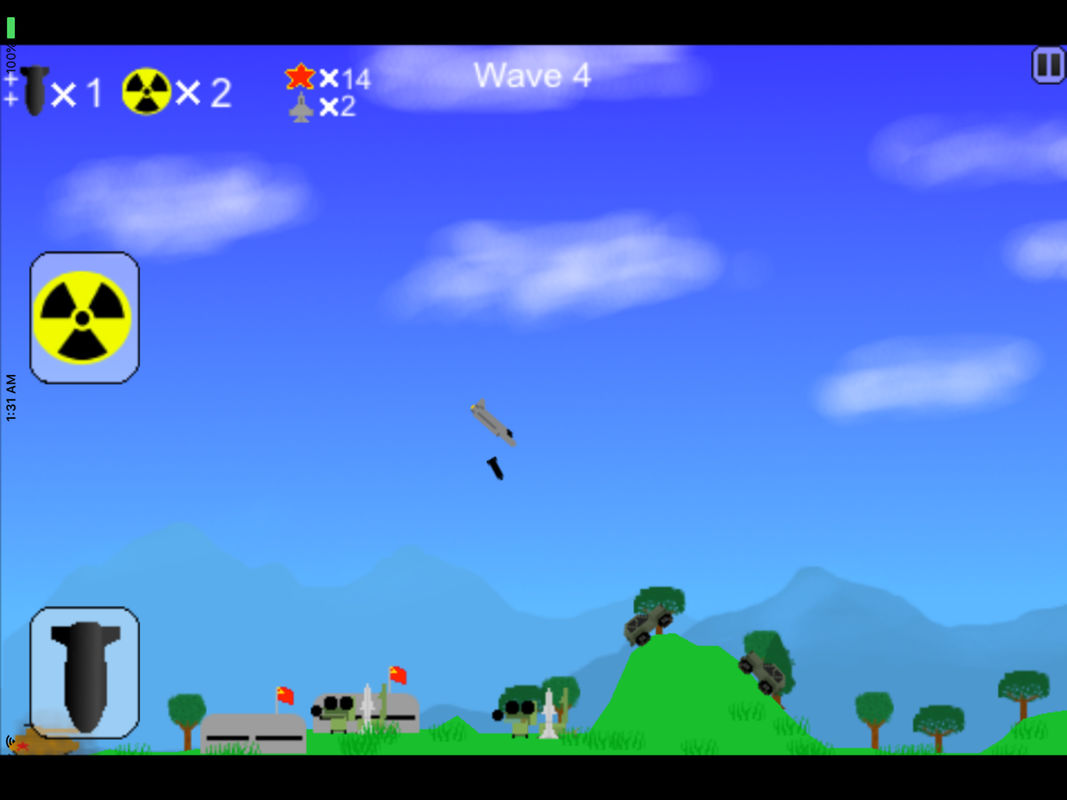
\includegraphics[width=\linewidth]{atomic-bomber}
				\caption{Скриншот игрового процесса оригинального <<Atomic Bomber>>}
				\label{atomic-bomber}
			\end{figure}
		\end{subsection}

		\begin{subsection}{Обзор инструментальных средств}
			Программа будет разработана на языке C++.
			Так как самостоятельная реализация даже самого базового графического фреймворка для разработки нашего приложения очень трудоемка, будем использовать движок Urho3D в качестве такого фреймворка.
			Он позволяет абстрагироваться от низкоуровневых деталей разработки игры, предоставляя реализации таких необходимых модулей как:
			\begin{enumerate}
				\item Управление жизненным циклом программы, обработка событий ОС.
				\item Компонентно-ориентированная модель для описания объектов в 2D/3D среде (сцене), легковесный визуальный редактор сцен.
				\item Загрузка текстур и других ассетов в различных форматах, рендеринг 2D и 3D графики, вывод звука, рассчет физики, обработка пользовательского ввода и другие важные подисистемы.
			\end{enumerate}

			Рассмотрим подробнее три парадигмы программирования, которые мы будем использовать:

			Объектно-ориентированное программирование - наиболее популярная парадигма программирования на данный момент, поддерживается C++ на языковом уровне.
			Данный подход позволяет моделировать предметную область как набор объектов, взаимодействующих друг с другом.

			Компонентно-ориентированное программирование - широко используемый при разработки игр подход, максимально использущий композицию вместо наследования (<<composition over inheritance>>).
			Существуют различные его вариации, но в данной работе мы будем использовать модель, предоставляемую движком Urho3D, в котором данный подход используется для описания структуры игровой сцены.
			Компонентно-ориентированный подход к построению сцены позволяет удобно реализовывать логику взаимодействия игровых объектов в 2D/3D пространстве и инкапсулировать отдельные ее аспекты.
			Объекты на сцене (называемые \verb|Node|) являются C++ классами, не предоставляющими сами по себе никакой функционал кроме их идентификации и координат на сцене, но при этом являющимися контейнерами компонентов.
			С помощью таких методов, как \verb|GetComponent<TComponent>| и \verb|AddComponent<TComponent>()|, программист может описывать функционал объекта набором ассоциированных с ним компонентов.
			Например, игровой ландшафт может быть представлен объектом с компонентами логической модели ландшафта, его физической модели и компонента отрисовки в спрайт.
			Сами компоненты также являются C++ классами, унаследованными от \verb|LogicComponent|.

			Событийно-ориентированное программирование - используемый в различных областях подход, описывающий систему как набор событий и действий, ассоциированных с активацией этих событий.
			В нашей программе мы будем использовать реализацию событий с помощью шаблона проектирования <<Наблюдатель>> (<<Observer>>) на основе указателей на функции C++ для коммуникации между компонентами объектов.
			Для этого воспользуемся открытой библиотекой Signals~\cite{signals}, предоставляющей функционал сигналов и слотов, похожий на делегаты и события в C\#.

			Для поддержания качества кода использовались диагностики IDE CLion и статический анализатор кода PVS-Studio.

			При разработке использовались порталы документация языка C++~\cite{cppreference}, API Urho3D~\cite{urho3d-docs}, а также книга, описывающая основные шаблоны проектирования Теплякова С~\cite{teplyakov}.
		\end{subsection}


	\end{section}

	\begin{section}{Программная реализация игры}

		\begin{subsection}{Инициализация}
			Входной точкой нашего приложения является класс GameApplication, который регистрируется в движке Urho3D макросом \verb|Urho3D_DEFINE_APPLICATION_MAIN(GameApplication)|.
			В нем производится получение контекста от Urho3D, начальная настройка приложения, вызов регистрации классов компонентов, а также создание и регистрация подсистемы управления игровым состоянием GameSubsystem (в Urho3D подсистемами называются объекты, существующие в единственном экземпляре во всем приложении).

			GameSubsystem предоставляет функционал загрузки, выгрузки и перезагрузки нашего игрового уровня.
			Компоненты на нем, в свою очередь, реагируют на различные события (например, переход на следующий кадр, пользовательский ввод или столкновения), формируя игровой процесс.
		\end{subsection}

		\clearpage
		\begin{subsection}{Структура уровня}
			Уровень (сцена) представляет собой иерархию объектов (называемых Node) и их компонентов:

			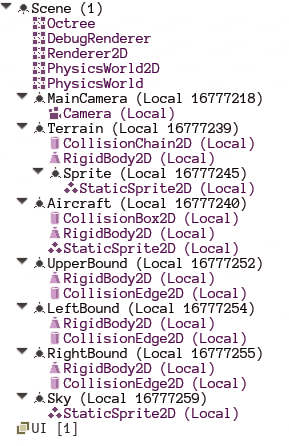
\includegraphics[width=250]{scene}

			\begin{enumerate}
				\item Объект MainCamera в нашем случае является закрепленной на одном месте ортогональной (не перспективной, т.к. наш мир двухмерен) камерой.
				Автоматически масштабируется при запуске для корректного отображения игровой области.
				\item Объект Terrain представляет ландшафт.
				\item Объект Aircraft представляет самолет игрока.
				\item Объект Sky отображает спрайт неба на заднем плане.
				\item Объекты LeftBound, RightBound и UpperBound расположены по краям видимой области и содержат физические коллайдеры, не позволяющие игроку покинуть пределы видимого пространства.
			\end{enumerate}

			Рассмотрим их подробнее.
		\end{subsection}

		\begin{subsection}{Ландшафт}
			Наиболее комплексная система в нашем приложении, состоит из трех компонентов
			\begin{enumerate}
				\item \verb|TerrainController| предоставляет логическую модель ландшафта, с которой работают другие компоненты.
				\item \verb|TerrainSpriteController| занимается динамической отрисовкой спрайта ландшафта.
				\item \verb|TerrainCollisionShapeController| выполняет динамическое построение физической модели ландшафта для работы столкновений.
			\end{enumerate}

			\verb|TerrainController| содержит карту высот: одномерный массив чисел с плавающей точкой, содержащий высоты в соответствующих точках ландшафта.
			Предоставляет методы для деформации ландшафта (взрыва), перевода координат из относительных координат (например, 0.5 будет серединой ландшафта) в абсолютные (мировые), а также событие об изменени ландшафта, позволяющее подписчикам отреагировать на это изменение.

			В начале игры карта высот генерируется одномерной версией алгоритма MidpointDisplacement, который рекурсивно генерирует случайную высоту в середине заданного промежутка на основании высот краев:
			\clearpage
			\inputminted{cpp}{listings/MidpointDisplacement1D.cpp}

			При любых изменениях карты высот вызывается событие \verb|HeightmapUpdated|, позволяющее указанным выше компонентам перерисовать спрайт и перестроить сетку коллизий.

			Пример генерируемого ландшафта приведен на рисунке~\ref{terrain}.

			\begin{figure}[h]
				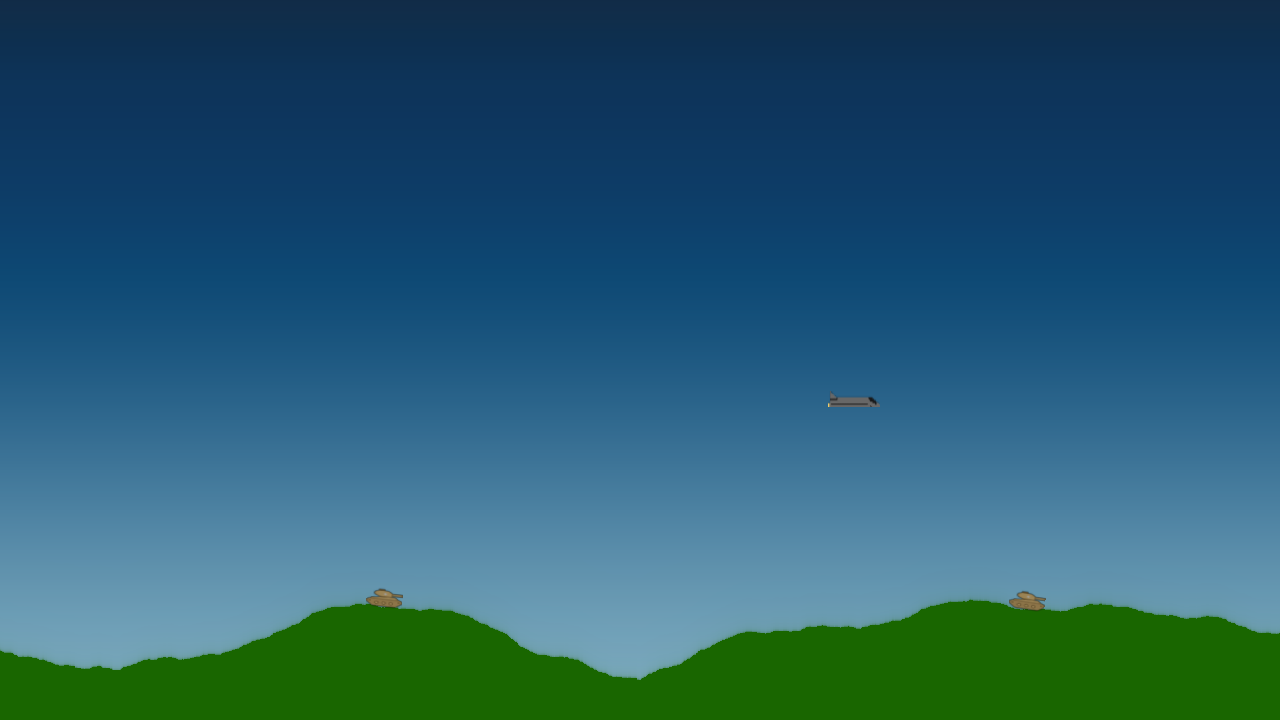
\includegraphics[width=\linewidth]{terrain}
				\caption{Пример сгенерированного ландшафта}
				\label{terrain}
			\end{figure}
		\end{subsection}

		\begin{subsection}{Игрок}
			Поведение самолета игрока контроллируют следующие компоненты:
			\begin{enumerate}
				\item \verb|AircraftController| подписывается на событие столкновения с ландшафтом (для вызова \verb|GameSubsystem::RequestReloadGameLevel| при столкновении), создает остальные компоненты.
				\item \verb|AircraftMovingController| контроллирует движение самолета: поддерживает скорость и направление движения, обрабатывает коллизиии с краями мира.
				\item \verb|AircraftMouseController| обрабатывает пользовательские клики мышью и отправляет соответствующие команды на изменение направления движения самолета (полет к заданной точке).
				\item \verb|AircraftBombsController| обрабатывает нажатие клавиши сброса бомб, инстанцирует объект бомбы.
			\end{enumerate}
		\end{subsection}

		\clearpage
		\begin{subsection}{Коллизии}
			Обработка коллизий ведется компонентом \verb|CollisionsAggregator|, который должен быть присутствовать у всех динамических объектов, заинтересованных в регистрации столкновений со статическим окружением.
			Оборачивает внутренние физические события Urho3D и предоставляет события, соответствующие каждому из типов коллайдеров (описаны далее).
			Например, так выглядит подписка самолета на свое столкновение с ландшафтом:

			\inputminted{cpp}{listings/AircraftCollisionExample.cpp}

			Для того, чтобы была возможность раздельно обрабатывать столкновения с тремя коллайдерами краев мира и ландшафтом, был введен базовый компонент \verb|StaticColliderComponent|, каждый из наследников которого идентифицирует свой тип коллайдера.

			Благодаря такому подходу, \verb|CollisionsAggregator| при регистрации столкновения просто проверяет наличие \verb|StaticColliderComponent| на столкнувшемся объекте и наличие идентификатора его конкретного типа в своем внутреннем словаре соответствующих событий.
			Если для этого типа коллайдера было создано событие во внутреннем словаре (\verb|HashMap|), то оно будет вызвано.

			Выделение этого функционала в универсальный компонент \verb|CollisionsAggregator| позволило избежать дублирования однотипного кода подписок на столкновения в компонентах самолета, бомб и т.д.
		\end{subsection}

		\begin{subsection}{Снаряды}
			При создании объекта бомбы на ней инициализируется компонент \verb|ShellController|, который в свою очередь обрабатывает движение и столкновения с границами мира, а также инициализирует компонент \verb|ExplosivesController|.
			Последний содержит характеристики взрыва и статическое событие \verb|SomethingExploded|, позволяющее таким объектам как ландшафт и противникам отреагировать на взрыв соответствующим образом.
			В частности, ландшафт деформируется, а противник будет уничтожен, если находится в радиусе.

			Такая событийно-ориентированная организация позволяет в дальнейшем прикрепить этот компонент не только к бомбам, но и к любым другим снарядам, в том числе и направленным против игрока.
			Потребуется лишь указать характеристики, а игроку подписаться на событие взрыва.
		\end{subsection}

		\begin{subsection}{Противники}
			На данный момент представлены только танками.
			Структура компонентов практически не отличается от самолета, но вместо контроля игроком выполняется простое движение влево/вправо с заданной скоростью с разворотом у границ мира.
		\end{subsection}

		\begin{subsection}{Тестирование}
			Проводились тесты на одновременный выброс большого количества бомб, в том числе и в пролете через границу мира.
			Также тестировалась многоразовая перезагрузка уровня в разных условиях.

			В процессе реализации логики ландшафта была обнаружена и исправлена утечка памяти в используемом внутри Urho3D физическом движке \verb|Box2D| (\url{https://github.com/Urho3D/Urho3D/issues/1995}).
			Обнаружить и локализовать проблему помог динамический анализатор кода \verb|Valgrind|.

			Также регулярно проводились проверки статическим анализатором кода PVS-Studio.
		\end{subsection}

	\end{section}

	\begin{section}{Заключение}
		В данной курсовой работе удалось реализовать запланированный функционал программы с использованием средства языка C++, а также различных библиотек и инструментов.

		Была использована на практике комбинация объектно-ориентированного, компонентно-ориентированного и событийно-ориентированного подходов программирования в совокупности с различными технологиями и инструментами разработки программного обеспечения.

		Исходный код проекта и текст данной работы доступны по адресу \url{https://github.com/ArXen42/AlienBomberUrho3D}.
	\end{section}

	~\nocite{urho3d-docs,cppreference, teplyakov}
	\printbibliography[title = Список использованных источников]

\end{document}
